\section{一个简单的Serverless平台原型(汪润川)}
\subsection{简述}
为了对 Serverless 计算有一个比较直观的认识,我们调研了一个供研究和测试用的 Serverless 平台原型\cite{mcgrath2017serverless}。该平台原型由 .NET 实现,部署在 Microsoft Azure 上,以 Windows 容器为函数执行环境。其基本架构如图\ref{figs:mcgrath2017_structure}所示,包括 Web 和 Worker 两个服务,中间消息层,以及代码和元数据存储平台。消息层和存储平台依赖 Azure Storage 实现。Web 服务暴露平台的公共 REST API,接收外部的调用消息,实现前后端的交互;一个 Worker 服务管理若干容器。
\begin{figure}[!htbp]
	\centering
	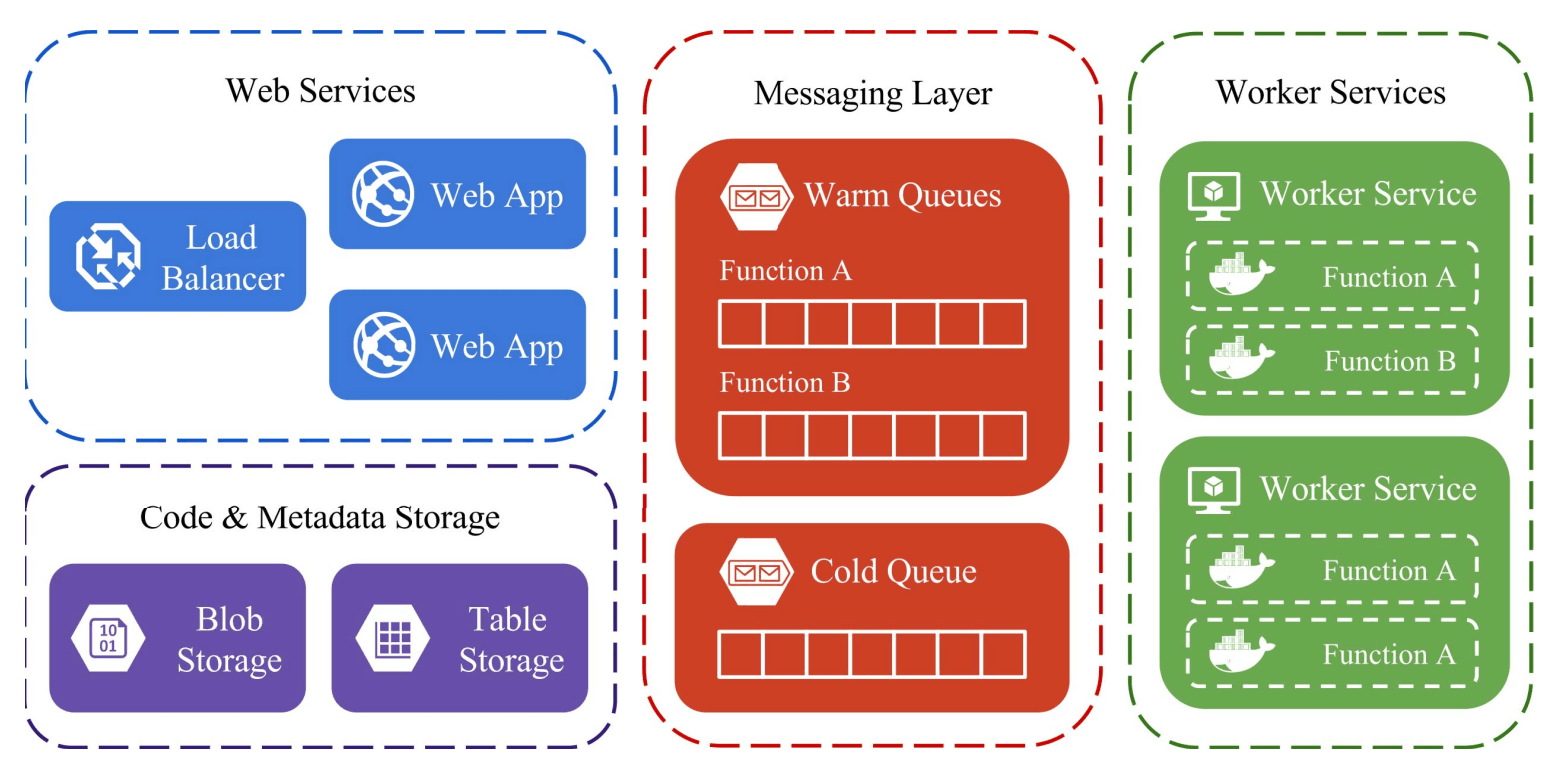
\includegraphics[width=0.9\linewidth]{figs/2017serverless_structure}
	\caption{Serverless 平台原型的基本架构。(\cite{mcgrath2017serverless}图1)}
	\label{figs:mcgrath2017_structure}
\end{figure}

\subsection{设计结构}
\subsubsection{函数元数据}
函数元数据(Function Metadata)是函数在执行过程中必须依赖的数据, 由四个部分构成:
\begin{enumerate}
	\item 函数标识符:全局唯一标识符(GUID),在函数创建时随机产生,用于唯一识别函数和函数资源。
	\item 语言运行时:规定了编写函数的语言。原型目前只支持 Node.js。
	\item 内存大小:决定了函数在容器内可以使用的最大内存容量。上限为 1 GB。
	\item 代码 Blob URI:函数的代码打包存储于云端平台,函数元数据记录 blob URI。
\end{enumerate}

\subsubsection{函数执行}
原型提供一个基本的函数执行模型,仅仅支持手动调用。当一个调用到达时,Web 服务首先接收调用信息(包括函数的输入),并从云端存储中获得函数元数据。输入和元数据共同构成函数的执行请求。Web 服务会尝试寻找 Worker 服务里可用的容器并提交执行请求。如果 Web 服务成功获得一个可用的容器, Worker 服务将执行函数并返回结果。


Web 服务和 Worker 服务之间通过一个共享的消息层进行联系。消息层中有两种队列:对所有函数一致的冷队列和每个函数独有的暖队列。队列中存储容器信息,包括 Worker 实例的地址以及容器名。冷队列中的容器没有被分配内存,使用时需要被启动。暖队列中的容器已经被分配内存,如果从队列中取到的容器刚好是空闲的,那么函数可直接使用。


Web 服务首先尝试从暖队列中获取一个空闲容器,如果不成功(可能暖队列为空,或者暖队列的首个容器正在被使用),则再从冷队列中获得一个容器,在 Worker 上部署和启动这个新容器。如果 Worker 的所有内存资源都被分配出去,那么冷队列为空。此时, Web 服务将无法在两个队列中获得可用的容器,会返回一个 HTTP 例外。冷队列反映了计算平台可用空间的多少,可以支持自动伸缩特性。

\subsubsection{容器分配}
每一个 Worker 管理自己的空闲内存池。若空闲的内存(既没有被分配也没有被预留的内存)大于函数可用的最大内存(1GB)时,这块大小为 1GB 的内存就会被预留。Worker 会为这块内存生成一个独有的容器名。此时,这块内存仅仅是被预留而非分配给容器和函数,因此内存信息和容器名会作为一个消息放入冷队列中。当一个冷队列中的容器需要被启动时,Worker 会根据函数元数据规定的内存大小真正的给容器分配内存,这时,这个容器的信息就由冷队列首转移到了暖队列尾。

\subsubsection{容器移除}
有两种情况容器会被移除。第一种情况是函数被删除,从而 Web 服务删除了函数的暖队列,Worker 则会定期监测暖队列的存在。第二种情况是容器被闲置超过15分钟。这两种情况下,Worker 会删除原函数所使用的容器并回收内存。回收的内存是空闲内存,当空闲内存超过函数可用的最大内存(1 GB)时,系统会预留容器,并向冷队列发送这个容器的消息。如果容器因函数闲置而被删除,当函数被再次调用时, Worker 服务会向函数返回 HTTP 例外,函数此时只能重新申请启动一个冷队列中的容器。

\subsubsection{容器镜像}
平台采用 Docker 运行容器,容器镜像包括函数运行时(目前只支持 Node.js)以及执行处理程序,而不包括任何函数代码。容器启动时,由平台在容器内附一个只读的函数代码,容器的可使用的内存资源也根据函数需要的内存大小进行分配。这样操作可以不用为每一个函数单独创建一个镜像,简单快捷。


容器的执行处理程序是一个简单的 Node.js 服务,它通过 HTTP 请求从 Worker 服务获取函数的输入,并给 Worker 返回函数的结果。

\subsection{评测结果}
作者将他设计的 Serverless 原型和市场上的主流 Serverless 计算平台进行了比较,包括 AWS Lambda, Azure Functions, Google Cloud Functions, Apache OpenWhisk。作者设计了两种测试方法:并发测试和退避测试。


并发测试评价系统的并发函数调用能力。测试工具在收到上一次函数的执行结果后,立即提交新的函数执行请求。测试开始时,一次只提交一个函数执行请求。每隔10秒增加一个并行函数,最多测试15个函数并行执行的效果。评测按照每秒收到的响应作为指标,评测结果如图\ref{figs:2017_concuttent_test}。
\begin{figure}[!htbp]
	\begin{subfigure}[b]{0.43\linewidth}
		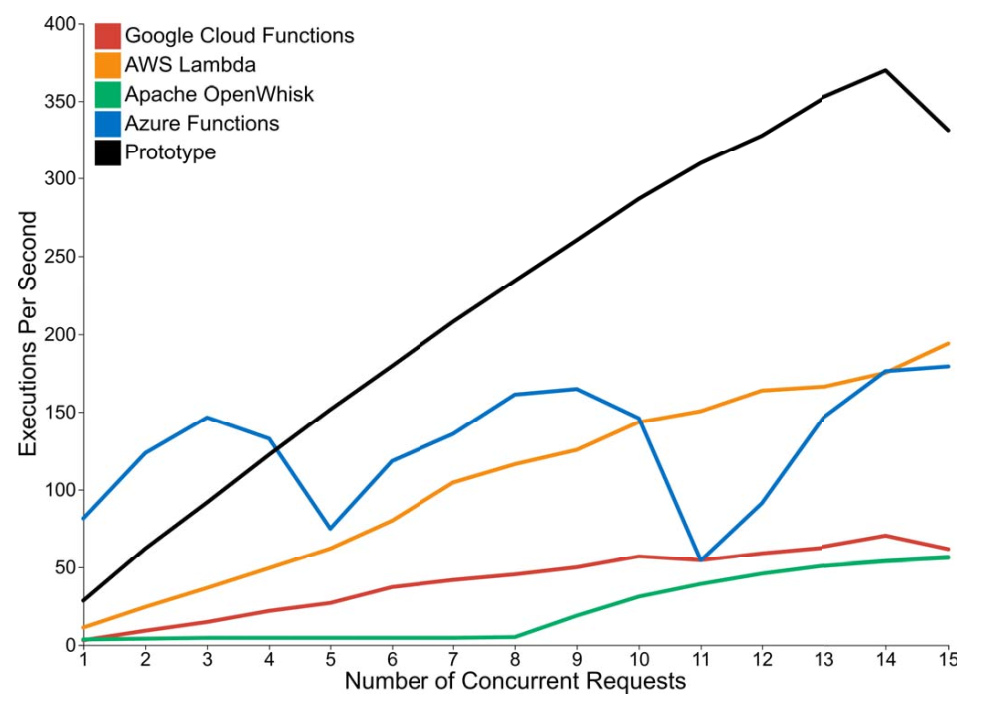
\includegraphics[width=\linewidth]{figs/2017_concuttent_test}
		\caption{}
		\label{figs:2017_concuttent_test}	
	\end{subfigure}
	\begin{subfigure}[b]{0.57\linewidth}
		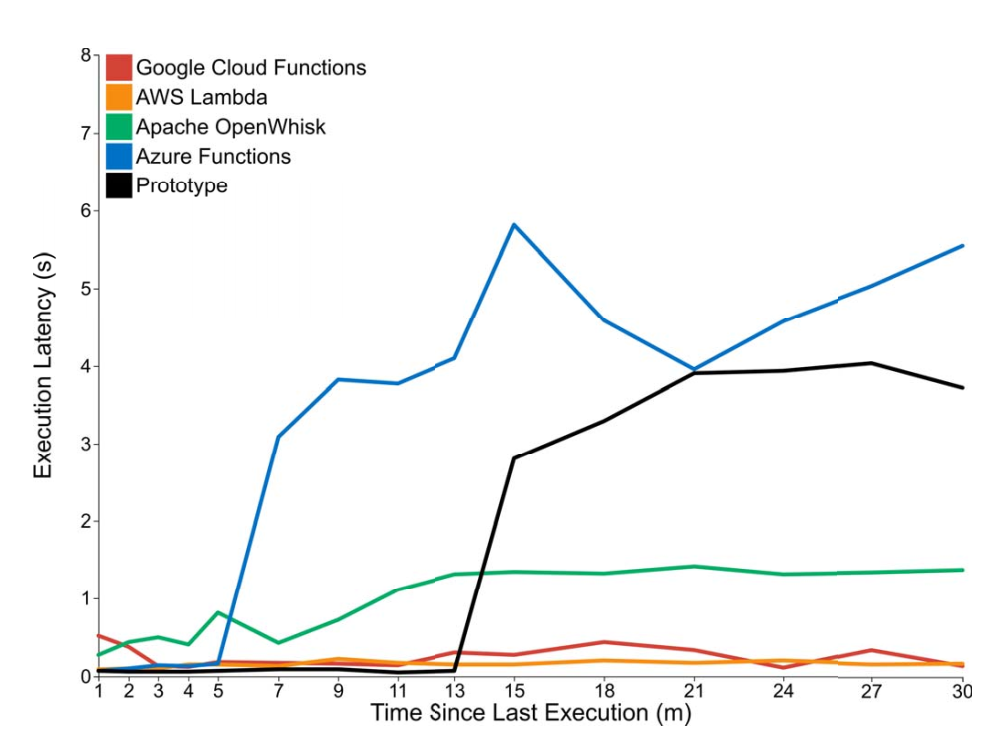
\includegraphics[width=0.8\linewidth]{figs/2017_backoff_test}
		\caption{}
		\label{figs:2017_backoff_test}
	\end{subfigure}
	\caption{(a) 并发测试结果。(b) 退避测试结果。(\cite{mcgrath2017serverless}图2、3)}
\end{figure}

在作者的平台上,如果并发函数小于15个,每秒执行次数与函数数量呈线性关系,但并发数为15时每秒执行次数下降。原因在于此时的负载已经接近单个 Azure 队列的伸缩极限,从而造成暖队列的延迟。其他的商用平台,AWS Lambda 的每秒执行数与函数数量呈线性关系,且有最高的吞吐量。 Google Cloud Functions 呈亚线性关系,并在15个并发函数处性能下降。 Azure Functions 呈波动关系。 OpenWhisk 在8个以下的并发函数都呈现低吞吐量,8个以上函数后呈亚线性关系,这可能是因为 OpenWhisk 的容器池会首选开启新的容器,而不是重新利用已开启的容器。

退避测试用于评价 Serverless 平台应对冷启动以及函数终止的表现。测试会按照递增的时间间隔向测试函数发送单个执行请求,时间间隔由1分钟向30分钟递增。测试结果如图\ref{figs:2017_backoff_test}。


再作者的平台上,根据设计,如果容器被闲置15分钟,那么它将会被收回,在这之后执行函数会遇到冷启动的问题。实验结果也反映出来,在15分钟后,原型的延迟会变得很高。Azure Functions 同样有着明显的冷启动问题。OpenWhisk 在10分钟之后会有轻微的冷启动问题,但和原型以及 Azure Functions 相比并不明显。Google Cloud Functions 和 AWS Lambda 几乎没有冷启动问题,可能是因为它们的容器启动时间短,或者容器在启动前有一个预分配内存的过程。

\subsection{讨论}
该 Serverless 原型还有如下的问题和可以改进的地方:
\begin{enumerate}
	\item 暖队列。已分配内存的容器放在队列中,会导致空闲容器堵塞的问题。一个容器即使执行完毕,如果在它之前分配的容器还没有执行完毕,那么这个容器并不能被 Web 看到并且使用。它必须等待之前分配的容器完成执行,或者自己闲置 15 分钟后被回收。这类问题需要栈或持续性哈希等结构的配合进行解决,然而 Azure 存储平台暂不支持这些数据结构。
	\item 异步执行。当前的平台只支持同步执行,即一个执行请求在提交之后必须等待函数执行完成,返回执行结果。异步执行允许执行请求只调用函数,不需要等待函数结果。异步执行的难点在于要保证至少一次执行。可以采用队列记录执行的函数,并增加一个监控服务,检测因平台问题而执行失败的函数,并重新执行。
	\item Worker 利用率。实际应用中, Worker 的资源通常会被过度分配,因为并非所有的函数都会持续执行,或是完全利用内存空间,这就涉及到执行效果和计算开销上的平衡。这个问题需要对大量的执行负载进行分析。
	\item Windows 容器。Windows 容器相比于 Linux 容器有着很大的不足。在平台原型中,Windows 容器无法在闲置的时候暂停,只能关闭和回收。另外,Windows 容器的可用资源必须在函数执行前配置好,无法在执行请求到达时再进行动态调整。
	\item 安全性。虽然容器已经被精心设计,函数权限也有限制,但将用户的所有代码托管在容器中依然是非常危险的行为。未来仍需要对函数执行环境的被攻击可能性进行评估。
	\item 测试方法。还有更多可以测试的内容,比如不同语言进行时的延迟比较、代码大小的延迟比较、系统事件类型比较、CPU 分配比例等等。
\end{enumerate}

作者的 Serverless 平台虽然比较简单,支持的功能也有限,但已经具有了一般 Serverless 平台的特点,包括函数驱动,自动部署,自动扩容缩容等。其遇到的问题,如冷启动,也是 Serverless 商用平台所需要解决的。

\section{Knative与Google Cloud Run(汪润川)}

\subsection{简述}
传统的 Serverless 存在着厂商绑定、缺乏行业标准的问题,为此,Google 联合 Redhat, IBM 等公司推出了 Knative 框架,旨在提供一套简单易用的 Serverless 计算方案,把 Serverless 标准化。它以分布式容器 Kubernetes 为基础,并提供了缩容到零、自动扩缩、集群内构建以及事件框架等功能。Knative 于2018年7月推出,目前仍在快速发展阶段。Google Cloud Run 是 Knative 的完全托管版本。

\begin{figure}[!htbp]
	\centering
	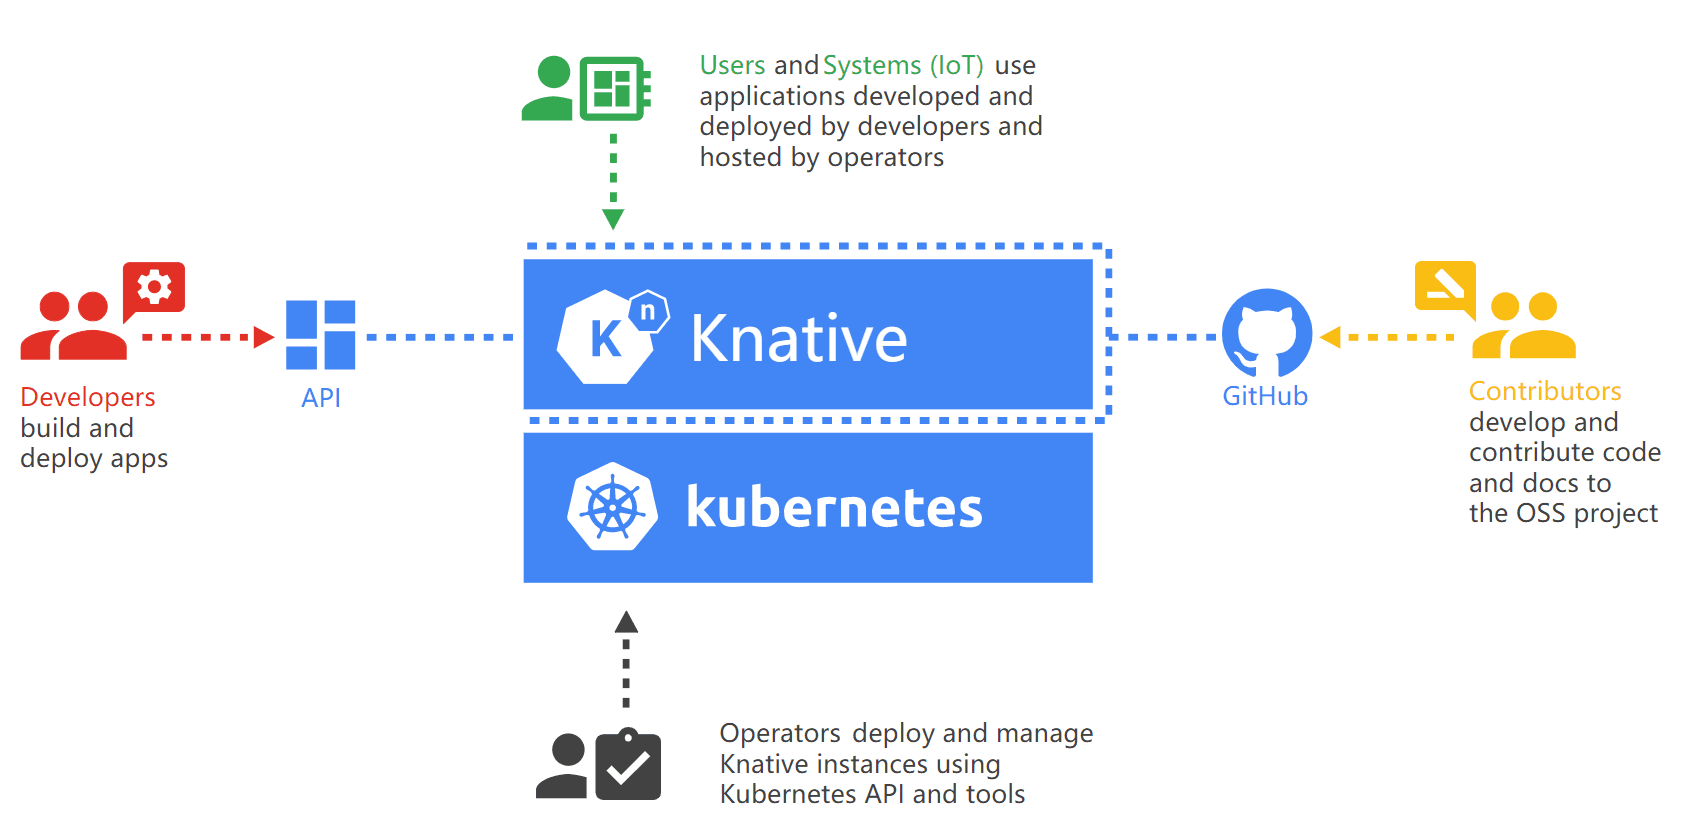
\includegraphics[width=1.0\linewidth]{figs/knative-audience}
	\caption{Knative 是基于 Kubernetes 的 Serverless 扩展。(\cite{knative-audiance})}
	\label{figs:knative-audience}
\end{figure}


Kubernetes(k8s)是自动化容器操作的开源平台,这些操作包括部署,调度和节点集群间扩展。Kubernetes 支持 Docker,Rocket 等容器技术。 Kubernetes 本身非常强大,但它十分复杂,开发人员需要理解并管理其丰富的资源,以及学习很多相关工具(yaml, kubectl, Istio, ...)。 Kubernetes 的理念与云原生(Cloud Native)背道而驰。Knative 是一个 Serverless 版的 Kubernetes ,使得开发人员可以只专注于业务代码而非基础设施。当然,如果 Knative 不能满足开发人员的需求,Knative 背后的 Kubernetes 功能依然可以被直接使用。下面简单介绍一些与 Knative 相关的 Kubernetes 概念。


Pod 是 Kubernetes 最小的调度单位,Pod 从属于 Node(物理机或虚拟机),Pod 中可以运行多个 Docker 容器,处于一个 Pod 中的多个容器共享共享网络和文件系统,以及 PID、IPC、Network 和 UTS 的命名空间\cite{k8s-pod}。Pod 在创建时会被分配一个IP地址,Pod 间的容器可以互相通信。Deployment 是 Pod 版本管理的工具,用来区分不同版本的 Pod。ReplicaSet 是副本控制器,使 Pod 副本数量始终维持在预设的个数。


Kubernetes 中的所有事物都被视为一个 API 对象并且都有一个与之对应的 API 入口。所有的操作和组件间的通信,包括外部的用户命令,都是由 API Server 处理的 REST API 调用。在 Kubernetes 中一切都可视为资源,系统提供了很多默认资源类型,如 Pod、Deployment等。一种资源就是 Kubernetes API 中的一个端点,它存储着某种 API 对象的集合。自定义资源(CRD)是对 Kubernetes API 的扩展,在一个运行中的集群内,自定义资源可以通过动态注册出现和消失,集群管理员可以独立于集群本身更新自定义资源\cite{k8s-CRD}。


Knative 包含2个核心组件: Serving 和 Eventing。Serving 提供 Serverless 应用或函数的部署能力以及各种服务管理,底层采用 Kubernetes 的 Pods;Eventing 管理进入到环境中的事件,提供事件触发的通道。事件不仅要被送达到相应的服务,也要被持久化到某些队列中去,以适应目标服务当前不可用的情况。同时,Knative 还依赖于 CI/CD 流水线 Tekton 完成从代码到部署的过程。

\subsection{Knative 组件}
\subsubsection{Tekton} \label{Tekton}
早期 Knative 采用一个专门的 Build 组件将源码构建成容器,Build 组件完全基于 Kubernetes 生态,用 Kubernetes CRD 的方式实现。Build 组件现已不再维护和推荐使用,当前推荐的构建组件是持续集成和持续部署(CI/CD)流水线 Tekton Pipelines。Tekton 以自定义资源的形式提供了一组 Kubernetes 扩展,用于定义流水线。图\ref{figs:knative-TektonPipeline}展示了 Tekton Pipelines 的 CRD\cite{knative-TektonPipeline},包括:
\begin{figure}[!htbp]
	\centering
	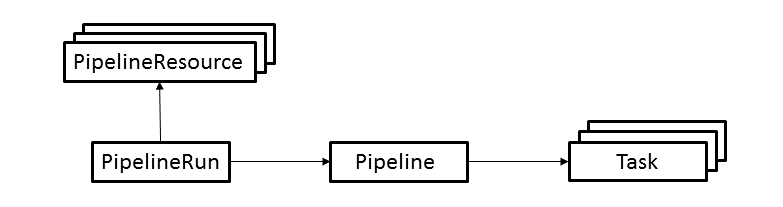
\includegraphics[width=0.8\linewidth]{figs/knative-TektonPipeline}
	\caption{Tekton CRD 结构。(\cite{knative-TektonPipeline})}
	\label{figs:knative-TektonPipeline}
\end{figure}
\begin{itemize}
	\item PipelineResource:定义了一个对象,该对象是流水线的输入(例如 git 存储库)或输出(例如 docker 镜像)。
	\item PipelineRun:定义了流水线的执行。它引用要运行的 Pipeline 以及要用作输入和输出的 PipelineResources。
	\item Pipeline:定义了构成流水线的 Tasks。
	\item Task:定义了一组构建步骤,如编译代码、运行测试以及构建和部署镜像,相当于一系列模板。
\end{itemize}

图\ref{figs:knative-source_to_image}展示了将一个应用从源码构建成容器镜像,然后再部署到 Knative 环境上的过程\cite{knative-source_to_image}。这个过程包括 Build (构建)和 Deploy (部署)两个 Tasks(任务),这两个任务通过一个 Pipeline 封装。 PipelineResource 包括了应用的源码,以及构建和部署会使用到的配置文件。 Build 阶段, kaniko (一款可以进行容器镜像构建的开源工具)会根据 Dockerfile 将源码构建成一个镜像,并上传到 Docker Registry 上。容器构建完成后, Build 会将镜像名、版本等信息传给 Pipeline 下游的任务。第二个任务同样从 PipelineResource 中获取部署的文件,利用 kuberctl (Kubernetes 的命令行工具)将 Docker Registry 上的镜像完成部署。

\begin{figure}[!htbp]
	\centering
	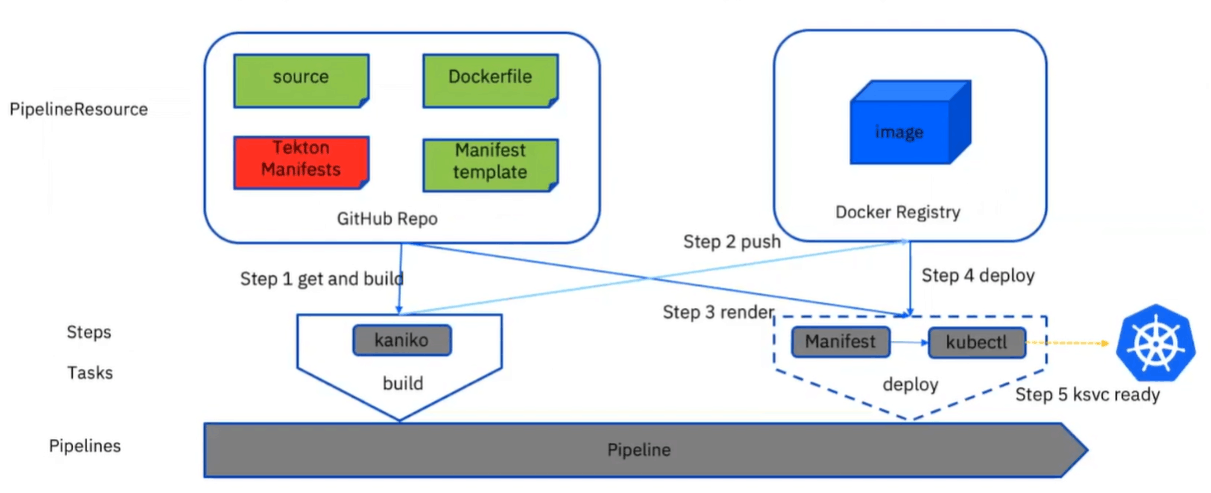
\includegraphics[width=1.0\linewidth]{figs/knative-source_to_image}
	\caption{利用 Tekton 从源码构建容器镜像。(\cite{knative-source_to_image}Page.12)}
	\label{figs:knative-source_to_image}
\end{figure}

\subsubsection{Serving}
Serving 提供了 Serverless 应用或函数的部署能力,以及自动缩扩容、版本管理、流量控制、滚动升级等功能。Serving 的基本结构如图\ref{knative-serving}所示,它提供四个主要的 API\cite{knative-servingapi}:
\begin{itemize}
	\item Route: 定义网络端口,映射一个或多个 Revision,将流量按比例导入不同的 Revision。
	\item Revision: 应用的旧版本,每次修改代码或配置的快照,可以根据进入的流量自动扩缩容。
	\item Configuration: 维护应用的最新配置,每次修改 Configuration 会产生一个新的 Revision。
	\item Service: 管理应用的整个生命周期,确保应用拥有 Configuration 和 Route。Service 可以被看作是正在部署的应用或者函数。
\end{itemize}
当需要进行滚动升级时,Route 会将所有流量逐渐路由到最新的版本中,而旧版本最终会因为没有流量而缩容至0。

\begin{figure}[!htbp]
	\begin{subfigure}[b]{0.48\linewidth}
		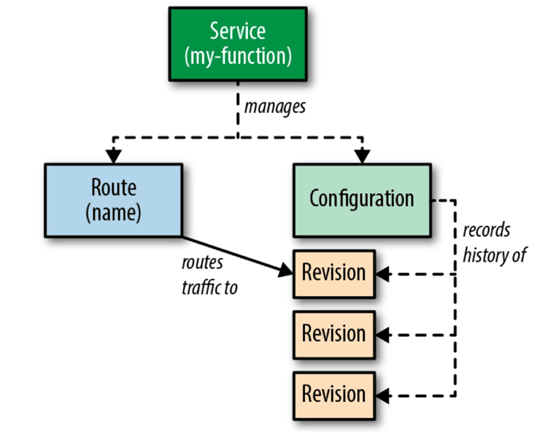
\includegraphics[width=\linewidth]{figs/knative-serving.png}
		\caption{}
		\label{knative-serving}
	\end{subfigure}
	\begin{subfigure}[b]{0.52\linewidth}
		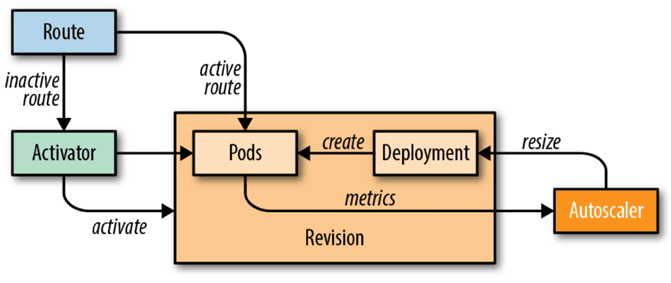
\includegraphics[width=\linewidth]{figs/knative-autoscaler.png}
		\caption{}
		\label{knative-autoscaler}
	\end{subfigure}
	\caption{(a) Serving 基本结构。(b) Autoscaler 实现自动缩容扩容。(\cite{mcclain2019getting}图2-1、2-2)}
\end{figure}

Revision 的自动缩容扩容功能还需要 Autoscaler 和 Activator 两个组件完成\cite{mcclain2019getting}。Reversion中的Pod会自动汇报metrics数据到 Autoscaler,Autoscaler 会根据请求量和资源使用情况修改Deployment的副本(replicas)数量,从而实现自动扩缩容。

Revision 处于激活状态才接受请求。当一个 Revision 停止接受请求时,Autoscaler将其置为待命状态。处于待命状态下,一个 Revision 底层部署缩容至零并且所有到它的流量均路由至 Activator。Activator 是一个共享组件,捕获所有到待命 Revision 的流量。当它收到某一待命 Revision 的激活请求后,它转变 Revision 状态至激活,然后代理请求至合适的 Pod。

\subsubsection{Eventing}
Knative Eventing 是一个旨在满足云原生开发的常见需求的事件平台,提供可组合的元素以支持后期绑定事件生产者和事件消费者。特征是松耦合、事件生产者和消费者互相独立、支持第三方服务接入、支持跨平台和互操作性\cite{knative-eventing}。


Eventing 定义了一组 Kubernetes CRD,包括
\begin{itemize}
	\item Event Source: 用于把事件生产者接入 Knative 事件平台,并把事件传送给消费者。
	\item Channel: 实现事件的转发和存储。底层实现可以有 Kafka, NATS Streaming 等。
	\item Subscription: 事件的订阅者,即事件转发的目的地。
	\item Parallel: 事件同时转发给多个订阅者,每个订阅者接收到同一个事件。
	\item Sequence: 事件依次经过多个订阅者,每个订阅者都可以修改,过滤或者创建新的事件。
	\item Broker: 可以接收事件,并将事件根据过滤条件转发给订阅者。
	\item Trigger: 根据订阅者的要求对事件设置过滤条件过滤。
	\item Event Registry: 用于查阅 Broker 中的事件类型。
\end{itemize}

Sink 是 Eventing 中一个重要概念,表示事件消息传送的目的地,也就是事件接收者的一个 HTTP 端口。


一个简单的事件订阅流程如图\ref{knative-cha_sub}所示。 Event Source 定义了事件源,通过 Sink 指定事件消费者的地址。 Knative 规定传输的事件必须符合 CloudEvents 格式,因此在 Event Source 后还有一个 Adapter(图中未画出)进行格式转换。为了适应单个事件源对多个订阅者的场景,需要使用 Channel 和 Subscription。 Channel 具有存储功能,可以避免消费者因暂时不在线而导致的消息丢失。 Subscription 连接 Channel 和消费者。消费者可以通过 Subscription 接收消息,也可以向 Subscription 发送回复,并由 Subscription 向其他 Channel 转发。基于 Channel 和 Subscription ,可以实现 Parallel 和 Sequence。
\begin{figure}[!htbp]
	\centering
	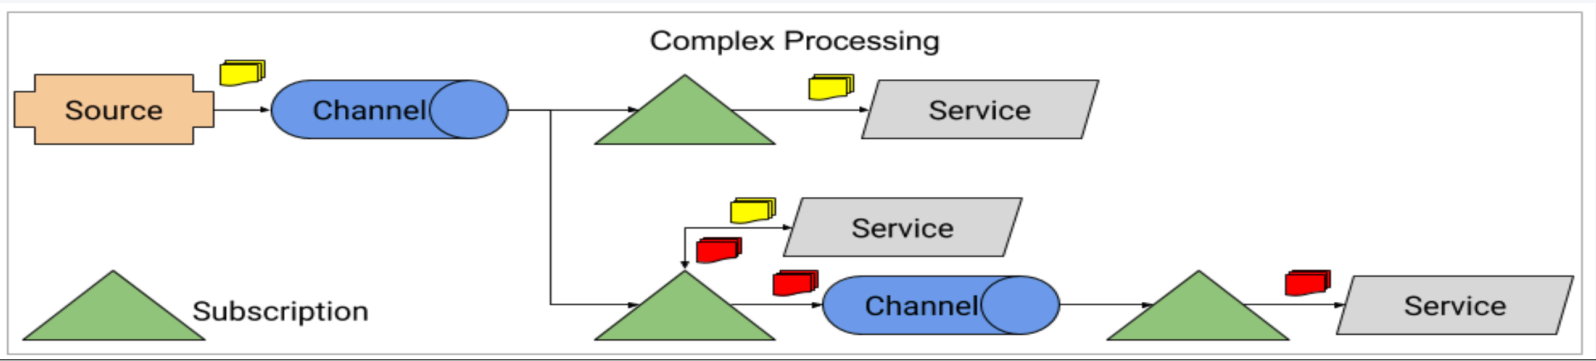
\includegraphics[width=\textwidth]{figs/knative-cha_sub.png}
	\caption{通过 Channel 和 Subscription 实现事件的转发和订阅。(\cite{knative-eventing}Page.18)}
	\label{knative-cha_sub}
\end{figure}

在较新的 Knative 版本中,Eventing 增加了 Broker 和 Trigger 对象,目的是搭建一个黑盒,将具体的实现隐藏起来,减少需要用户添加的 Channel 和 Subscription。同时, Broker 和 Trigger 可以满足消费者对信息过滤的需求,消费者可以选择订阅自己感兴趣的事件,而非接收 Channel 中的所有信息。Eventing 支持的过滤指标包括事件类型和来源,以及任何其他的事件属性。

\begin{figure}[!htbp]
	\centering
	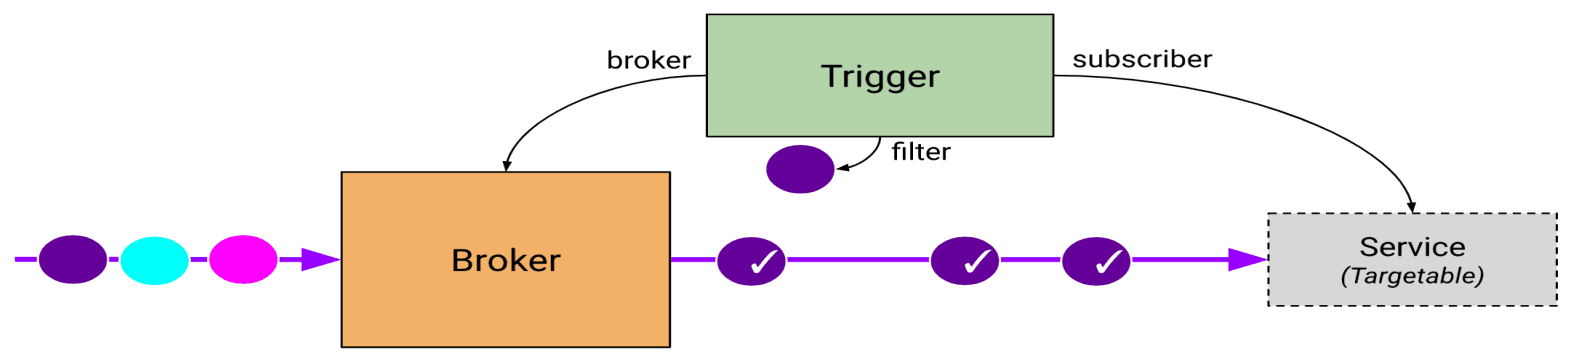
\includegraphics[width=\textwidth]{figs/knative-broker_2.png}
	\caption{通过 Broker 和 Trigger 实现事件的转发和订阅。订阅者告诉 Trigger 只要紫色的消息。Broker 对消息进行过滤,将紫色的消息发送给订阅者。(\cite{knative-eventing}Page.23)}
	\label{knative-broker}
\end{figure}
消费者此时不需要创建 Subscription 对象,而是创建一个 Trigger 对象,描述自己感兴趣的事件。Broker 是一个事件桶,接收各种事件,根据 Trigger 中定义的规则,对事件进行过滤,过滤之后发送给事件的订阅方。事件的转发和订阅结构如图\ref{knative-broker}所示。

\subsubsection{gVisor}
gVisor 是 Google 发布的沙箱技术,用于安全隔离宿主机和应用程序,提供比容器更为安全的隔离机制。gVisor 可以与 Docker 和 Kubernetes 集成在一起。Knative 的容器实际运行于与 Kubernetes 集成的 gVisor 上。在 Kubernetes 中,大多数资源隔离以 Pod 位单位,因此 Pod 也是 gVisor 沙箱的边界\cite{knative-gvisor}。gVisor为 Cloud Run 带来了安全容器的隔离,但是也带来了一些限制,例如,gVisor 支持的系统调用是有限的\cite{cloudrun_contract}。
\begin{figure}[!htbp]
	\centering
	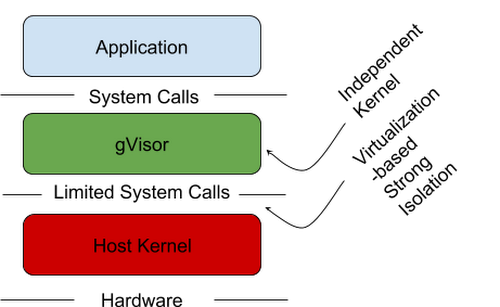
\includegraphics[width=0.7\textwidth]{figs/knative-gvisor.png}
	\caption{gVisor 支持的系统调用是有限的。(\cite{knative-gvisor}图3)}
	\label{knative-gvisor}
\end{figure}

\subsection{实际操作:构建和部署}
在这一节中,我们将根据 Google Cloud Run 文档中的教程\cite{cloudrun}构建和部署一个简单的 Hello-World python 应用,从程序员的视角体验 Knative 给开发带来的便利。Cloud Run 对运行的容器有如下要求和限制\cite{cloudrun_contract}:
\begin{itemize}
	\item 容器必须是 64 位 Linux 平台。
	\item 在 8080 端口监听 HTTP 请求。
	\item 容器必须在收到请求 4 分钟之内启动 HTTP 服务器。
	\item 每个容器默认可使用 256 MB 内存,最多可以使用 2GB 内存。
\end{itemize}

下面开始准备工作,首先注册 \href{https://cloud.google.com/}{Google Cloud} 账号。注册时需要提供信用卡信息,首次注册可以获得1年的免费使用期和 300 美元赠金。注册成功后打开 \href{https://console.cloud.google.com/}{Google Cloud 控制台},点击上方选择项目按钮,在弹出的对话框中选择“新建项目”,给新项目命名(如图\ref{figs:name}),系统会自动生成一个项目ID。创建项目后,为新创建的 Hello-World 项目启用 Cloud Build API,如图\ref{figs:start}。
\begin{figure}[!htbp]
	\begin{subfigure}[b]{0.5\linewidth}
		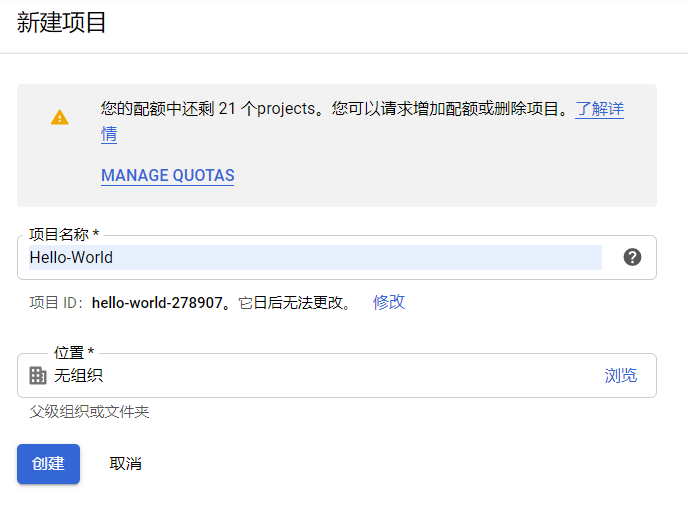
\includegraphics[width=\linewidth]{figs/cloudrun_name.png}
		\caption{}
		\label{figs:name}
	\end{subfigure}
	\begin{subfigure}[b]{0.5\linewidth}
		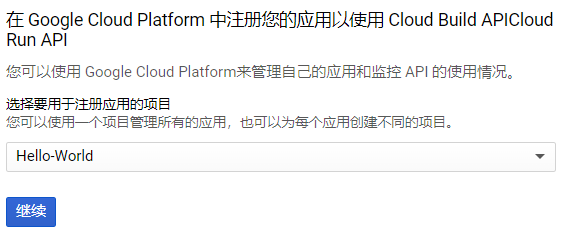
\includegraphics[width=\linewidth]{figs/cloudrunstartapi.png}
		\caption{}
		\label{figs:start}
	\end{subfigure}
	\caption{(a) 创建新的项目。(b) 启动 Cloud Build API。}
\end{figure}

在本地机器上安装和初始化 \href{https://cloud.google.com/sdk/docs}{Google Cloud SDK} \footnote{即使开了网络代理,Cloud SDK 在中国大陆地区的初始化也会遇到网络连接失败的问题。虽然可以在 Cloud SDK 中再配置代理信息,但为了方便起见,我直接在海外服务器上安装 Cloud SDK。因此,海外服务器是我开发的本地环境。}。Cloud SDK 是 Google Cloud 的命令行工具,用于访问 Google Cloud 的相关资源。Linux 系统下,Cloud SDK 的安装依赖于 Python 3。运行初始化 Cloud SDK 的命令
\begin{lstlisting}
# gcloud init
\end{lstlisting}
初始化阶段需要登录 Google Cloud 账号以及选择默认的项目。
在本地环境中编写应用代码:
\lstinputlisting[
%style = Python,
caption = {app.py}
]{./code/app.py}

此代码使用“Hello Bigdata”响应请求,以8080为监控端口。根据\ref{Tekton}节的部署要求,我们还需要创建一个 Dockerfile 作为容器的配置信息:
\lstinputlisting[
%style = Python,
caption = {Dockerfile}
]{./code/Dockerfile}

添加一个 .dockerignore 文件,以从容器映像中排除文件:
\lstinputlisting[
%style = Python,
caption = {.dockerignore}
]{./code/.dockerignore}

\begin{figure}[!htbp]
	\centering
	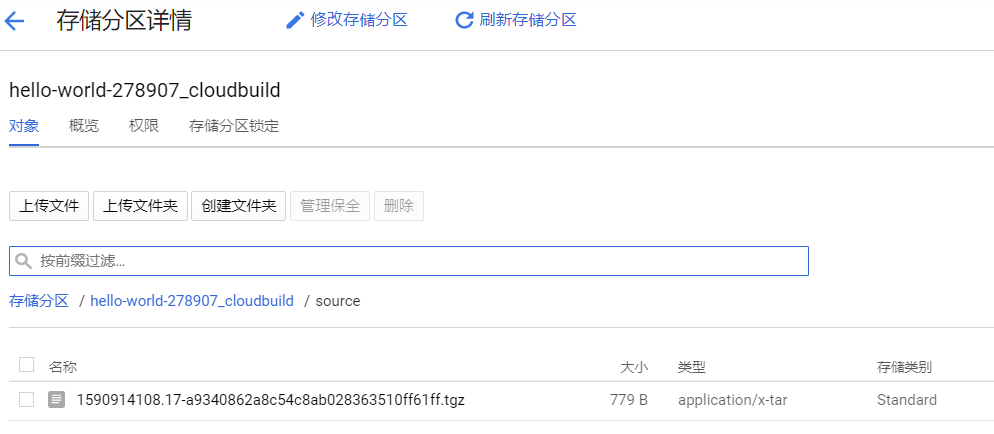
\includegraphics[width=0.8\textwidth]{figs/cloudrun_submit.png}
	\caption{代码和配置信息已被上传。}
	\label{cloudrun_submit.png}
\end{figure}
\begin{figure}[!htbp]
	\centering
	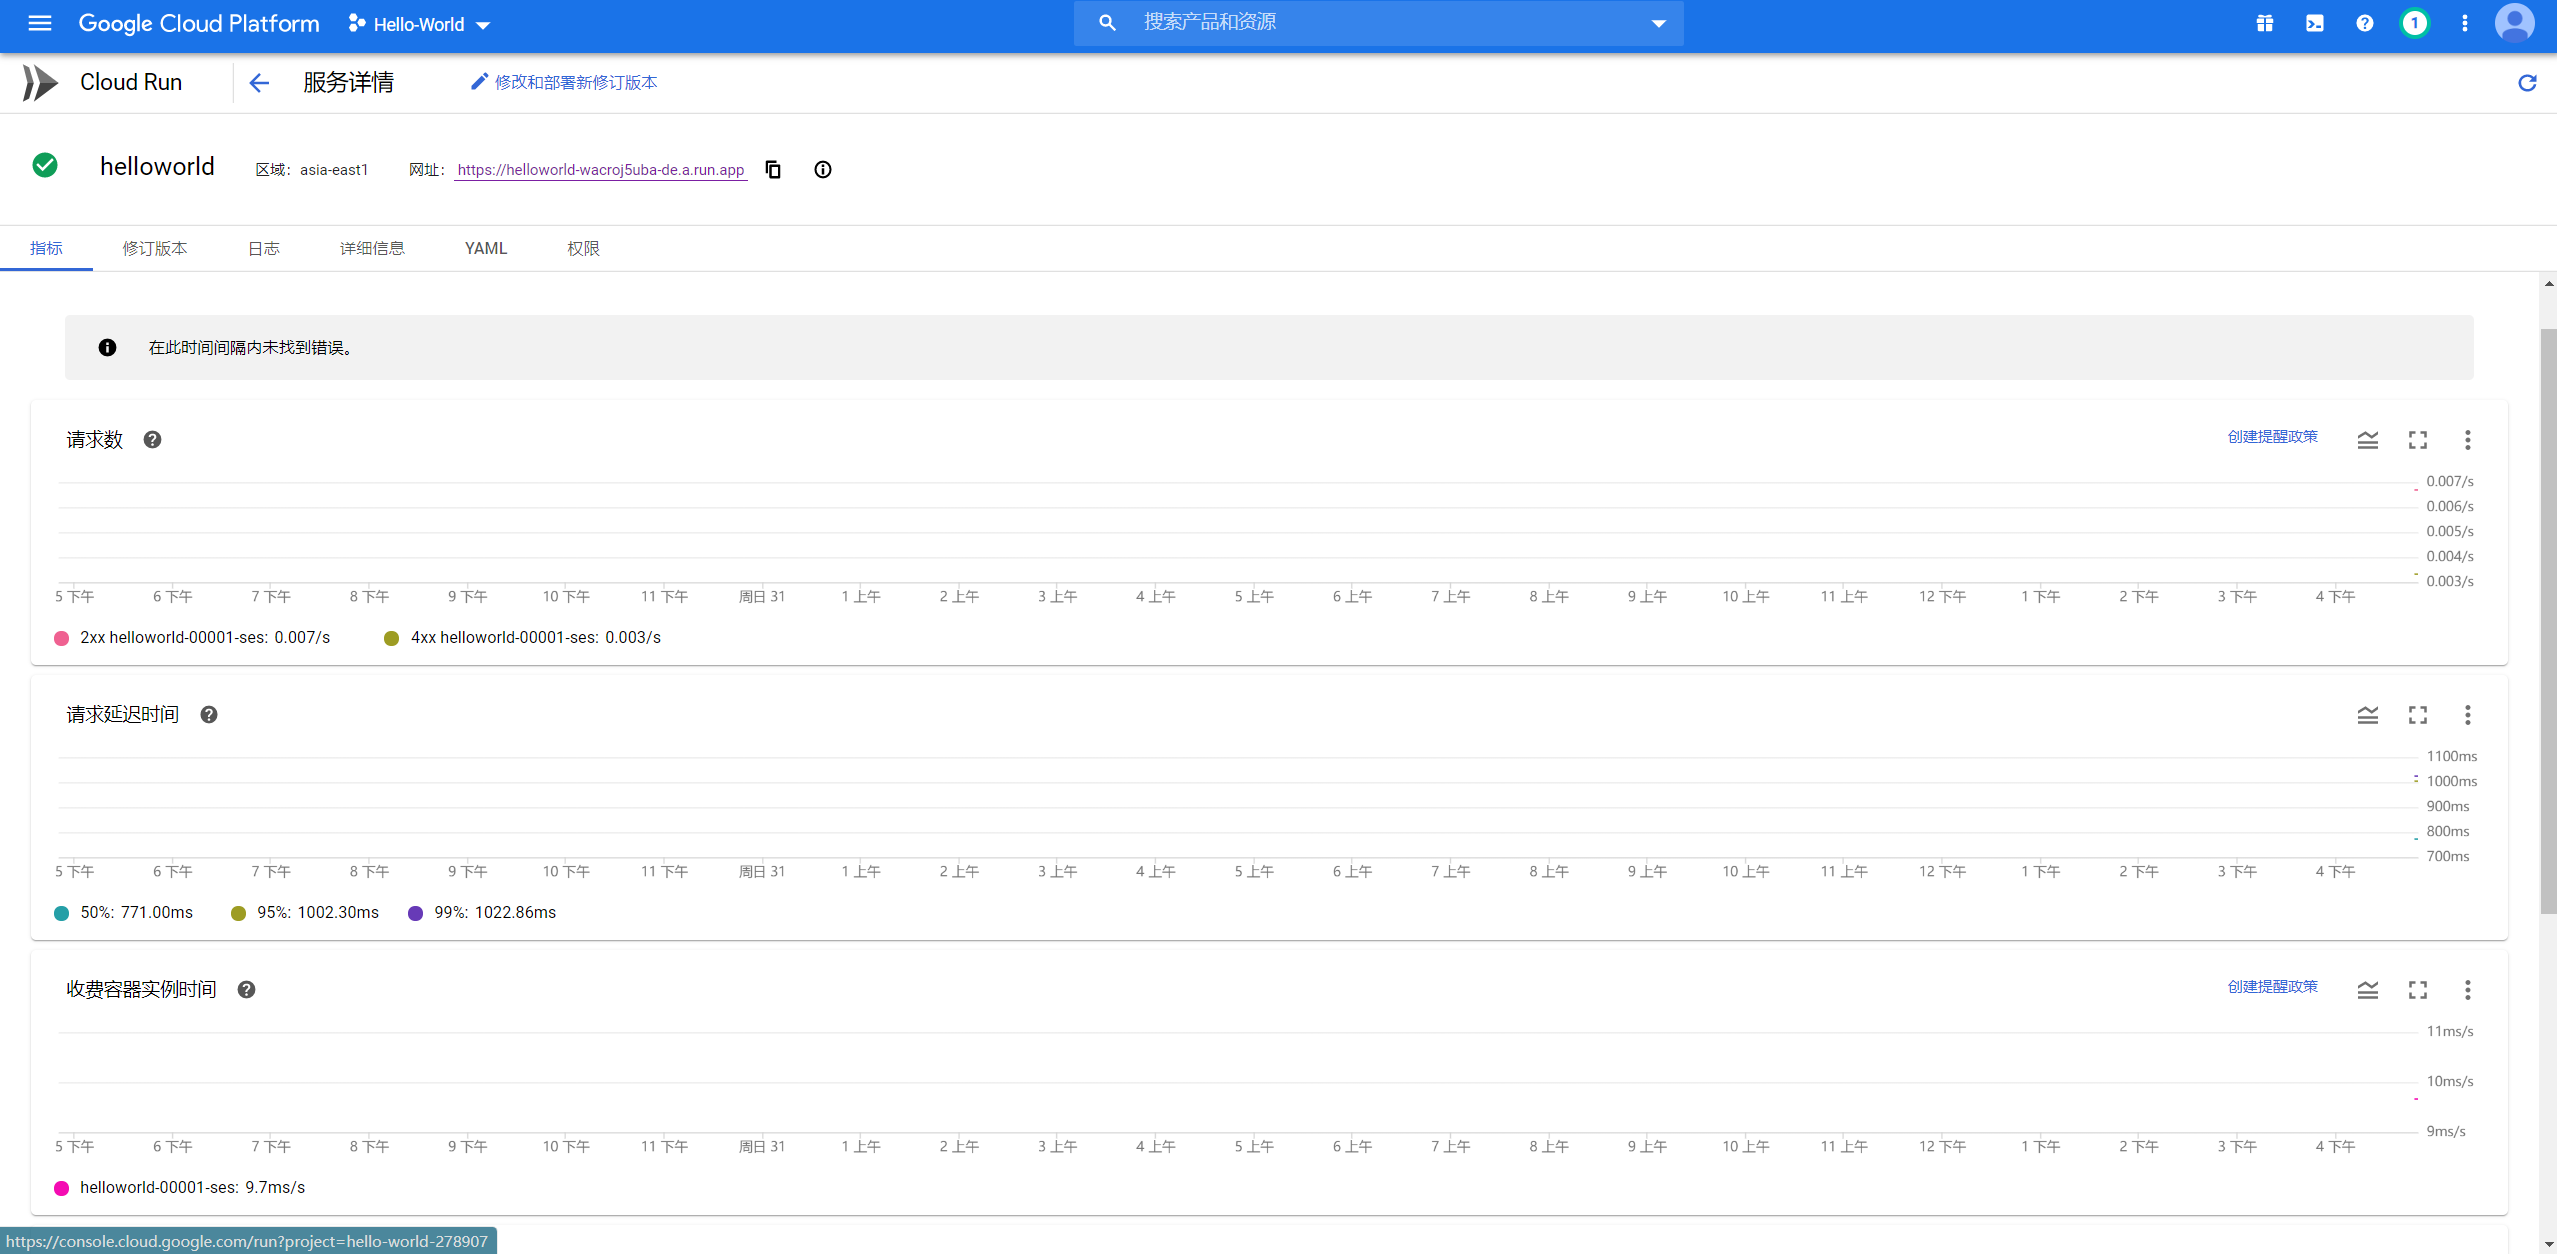
\includegraphics[width=0.8\textwidth]{figs/cloudrun_complete.png}
	\caption{Cloud 控制台可以监控服务的请求数、延迟时间、收费容器实例时间、容器的 CPU 和内存利用率。也可查看服务的版本、日志、权限等信息。}
	\label{cloudrun_complete.png}
\end{figure}

将这三份代码放在一个目录下,在这个目录下执行命令:
\begin{lstlisting}
# gcloud builds submit --tag gcr.io/hello-world-278907/helloworld
\end{lstlisting}
将代码和配置文件上传到 Container Registry 上并构建容器。其中,hello-world-278907 是项目 ID。通过 Google Cloud 控制台,可以看到代码和配置信息已被上传,如图\ref{cloudrun_submit.png}所示。

执行部署命令:
\begin{lstlisting}
# gcloud run deploy --image gcr.io/hello-world-278907/helloworld --platform managed
\end{lstlisting}
输入服务名称,选择部署服务器的位置。等待部署完成,命令行会显示服务网址。我部署的这个服务网址为\url{https://helloworld-wacroj5uba-de.a.run.app/},通过浏览器访问该地址,可以看到“Hello Bigdata!”的问候语。通过控制台,可以监控服务的各项指标,如图\ref{cloudrun_complete.png}所示。

在这个创建和部署的整个过程中,我们只写了应用代码和容器的配置信息,创建和部署只需要一条命令即可执行,非常方便快捷。

